\documentclass{article}

\usepackage{hyperref} %BUG if put after
\usepackage{tikz}
\usetikzlibrary{calc,shapes,positioning}
\usetikzlibrary{arrows}
\newcommand{\midarrow}{\tikz \draw[-triangle 90] (0,0) -- +(.1,0);}
% Be sure to use PDxF Latex
\pdfoutput=1

\usepackage[latin1]{inputenc}

\usepackage{url}
\usepackage{fullpage}
\usepackage{cite}
\usepackage{caption}
\usepackage{bm}
\newcommand{\ubar}[1]{\mkern2mu\underline{\mkern-2mu #1\mkern-2mu}\mkern2mu}
% \allowdisplaybreaks
\usepackage{mystyle}
\newcommand{\ubm}[1]{\ubar{\bm{#1}}}
\newcommand{\ubmr}[2]{\ubar{\bm{#1}}^{(#2)}}


% \newcommand{\bmtr}[3]{\bm{#1}^{(#3)}_{#2}}

\newcommand{\bmtr}[3]{\bm{#1}^{(#3)}_{#2}}
\newcommand{\smtr}[3]{{#1}^{(#3)}_{#2}}


\usepackage{amsmath,graphicx}
% format A4
% \usepackage{vmargin}
% \setpapersize{A4} 


\graphicspath{{./images/}}


\hypersetup{  
  bookmarks=true,
  backref=true,
  pagebackref=false,
  colorlinks=true,
  linkcolor=blue,
  citecolor=red,
  urlcolor=blue,
  pdftitle={Generative Model HMM},
  pdfauthor={Dong Liu},
  pdfsubject={}
}



\title{Powering Hidden Markov Model by Generative Models}
\author{
  Firsthand Scientists
}

% \name{
% Dong Liu,
% Minh Th�nh Vu,
% Saikat Chatterjee,
% and Lars~K. Rasmussen
% }

%   \address{
%   KTH Royal Institute of Technology, Stockholm, Sweden \\
%   E-mail: \{doli, mtvu, sach, lkra\}@kth.se}

\begin{document}

\maketitle
\section{Notation}
Time is indexed by subscript and sequence is denoted by underline. $\bm{x}_t$ is signal at time $t$. The sequential time is denoted by $\ubar{\bm{x}} = \left[ \bm{x}_1,
  \cdots, \bm{x}_T\right]^{\intercal}$, where $[\cdot]^{\intercal}$ means transpose and $T$ is the length of the sequence.  Sequential signal or clip uses underline notation and is indexed by superscript, for instance $\ubar{\bm{x}}^{(r)}$ means the $r$-th sequential signal, where $r = 1, 2, \cdots, R.$, and $\ubmr{x}{r} = \left[ \bmtr{x}{1}{r}, \bmtr{x}{2}{r}, \cdots, \bmtr{x}{T^{(r)}}{r} \right]$ with length ${T^{(r)}}$. Note different sequential signal $\ubmr{x}{r}$ could have different lengths.

The hypothesis of Hidden Markov Model (HMM): $\Hh := \{\bm{H} | \{\Ss, \bm{q}, A, p(\ubar{\bm{x}}|\ubar{\bm{s}}; \bm{\Phi})\}$,
\begin{itemize}
\item $\Ss$ is the set of states of HMM $\bm{H}$;
\item $\bm{q} = \left[ q_1, q_2, \cdots, q_{|\Ss|}\right]^\intercal$ initial distribution of HMM $\bm{H}$ with $|\Ss|$ is cardinality of $\Ss$, $q_k = p(s=k)$ for random state variable $s$.
\item $A$ is the transition matrix for the HMM $\bm{H}$ of size $|\Ss| \times |\Ss|$.
\item Observable signal density $p(\ubar{\bm{x}}|\ubar{\bm{s}};\bm{\Phi})$ given hidden state sequence, where $\bm{\Phi}$ is the parameter set that defines this conditional probabilistic model.
\end{itemize}

\section{Problem Statement}
Given a empirical distribution $\hat{p}(\ubm{x}) = \frac{1}{R}\sum_{r=1}^{R} \delta_{\ubmr{x}{r}}(\ubm{x})$. We want to find a probabilistic model such that:
\begin{equation}
  \min KL(\hat{p}(\ubm{x})\| p(\ubm{x}))
\end{equation}
where $KL(\cdot\|\cdot)$ denotes the Kullback-Leibler divergence.

When we use HMM to model the empirical distribution and approach the unknown true distribution, the problem boils down to:
\begin{equation}
  \uargmax{\bm{H} \in \Hh} p(\ubm{X}; \bm{H})
\end{equation}
where $\ubm{X} = \left[ \ubmr{x}{1}, \ubmr{x}{2}, \cdots, \ubmr{x}{R} \right]$ 

The problem can be reformulated as
\begin{equation}\label{eq:ml-of-hmm}
  \uargmax{\bm{H} \in \Hh} \sum_{r=1}^{R}\log\,p(\ubmr{x}{r}; \bm{H})
\end{equation}
for independent identical distributed assumption of $\ubm{x}$.

\section{Proposal}


Since model $\bm{H}$ contains hidden sequential variable $\ubm{s}$, we can not directly solve the maximum likelihood problem in $\autoref{eq:ml-of-hmm}$. We use expectation maximization (EM) to address the hidden variable problem by
\begin{itemize}
\item E-step: % the posterior probability of $\ubm{s}$:
  % \begin{equation}
  %   p(\ubm{s}|\ubm{x})
  % \end{equation}
  The ``expected likelihood'' function:
  \begin{equation}\label{eq:em-q-funciton}
    \Qq(\bm{H}; \bm{H}^{\mathrm{old}}) = \ \sum_{r=1}^{R}EE_{p(\ubmr{s}{r}| \ubmr{x}{r}; \bm{H}^{\mathrm{old}})}\left[\log\,p(\ubmr{x}{r}, \ubmr{s}{r}; \bm{H}) \right]
  \end{equation}
\item M-step: the optimization step:
  \begin{equation}\label{eq:em-m-opt}
    \umax{\bm{H}} \Qq(\bm{H}; \bm{H}^{\mathrm{old}})
  \end{equation}
\end{itemize}


The \autoref{eq:em-m-opt} can be reformulated as:
\begin{equation}\label{eq:m-step-subs}
  \umax{\bm{H}} \Qq(\bm{H}; \bm{H}^{\mathrm{old}}) = \umax{\bm{q}}\Qq(\bm{q}; \bm{H}^{\mathrm{old}}) + \umax{{A}}\Qq({A}; \bm{H}^{\mathrm{old}}) + \umax{\bm{\Phi}}\Qq(\bm{\Phi}; \bm{H}^{\mathrm{old}})
\end{equation}
where
\begin{align}
  \Qq(\bm{q}; \bm{H}^{\mathrm{old}}) &= \sum_{r=1}^{R} \EE_{p(\ubmr{s}{r}| \ubmr{x}{r}; \bm{H}^{\mathrm{old}})} \left[\log\,p(\smtr{s}{1}{r}; \bm{q})\right] \label{eq:init-distribution-update}\\
  \Qq({A}; \bm{H}^{\mathrm{old}}) &= \sum_{r=1}^{R} \EE_{p(\ubmr{s}{r}| \ubmr{x}{r}; \bm{H}^{\mathrm{old}})} \left[\log\,\sum_{t=1}^{T^{(r)}-1}p(\smtr{s}{t+1}{r}|\smtr{s}{t}{r}; {A})\right] \label{eq:transition-update}\\
  \Qq(\bm{\Phi}; \bm{H}^{\mathrm{old}}) &= \sum_{r=1}^{R} \EE_{p(\ubmr{s}{r}| \ubmr{x}{r}; \bm{H}^{\mathrm{old}})} \left[\log\,p(\ubmr{x}{r} | \ubmr{s}{r}; \bm{\Phi})\right]\label{eq:generative-model-update}
\end{align}

We can see that the solution of $H$ depends on the posterior probability $p(\ubm{s}| \ubm{x}; \bm{H})$. Though the evaluation of posterior according to Bayesian theorem is simple, the computation complexity of $p(\ubm{s}| \ubm{x}; \bm{H})$ grows exponentially with the length of $\ubm{s}$. Therefore, we would employ Forward/Backward algorithm \cite{} to do the posterior computation efficiently. The marginal $p(s_t| \ubm{x}; \bm{H})$ is also efficiently computed as the joint posterior. 


\subsection{Initial Probability Update}
\autoref{eq:init-distribution-update} can be written as:
\begin{align}
  \Qq(\bm{q}; \bm{H}^{\mathrm{old}}) &= \sum_{r=1}^{R}\sum_{\ubmr{s}{r}} {p(\ubmr{s}{r}| \ubmr{x}{r}; \bm{H}^{\mathrm{old}})} \log\,p(\smtr{s}{1}{r}; \bm{q}) \nonumber \\
                                     & = \sum_{r=1}^{R}\sum_{\smtr{s}{1}{r}=1}^{|\Ss|}\sum_{\smtr{s}{2}{r}=1}^{|\Ss|}\cdots \sum_{\smtr{s}{T^{r}}{r}}^{{|\Ss|}} {p(\smtr{s}{1}{r}, \smtr{s}{2}{r}, \cdots, \smtr{s}{T^{r}}{r}| \ubmr{x}{r}; \bm{H}^{\mathrm{old}})} \log\,p(\smtr{s}{1}{r}; \bm{q}) \\
                                     & = \sum_{r=1}^{R}\sum_{\smtr{s}{1}{r}=1}^{|\Ss|}{p(\smtr{s}{1}{r}| \ubmr{x}{r}; \bm{H}^{\mathrm{old}})} \log\,p(\smtr{s}{1}{r}; \bm{q}) 
\end{align}

Since $p(\smtr{s}{1}{r}; \bm{H})$ is the probability of initial state of HMM $\bm{H}$ for $r$-th sequential, actually $q_i = p(\smtr{s}{1}{r} =i;\bm{H} ) $ for $i= 1, 2, \cdots, |\Ss|$. Solution to problem:
\begin{align}
  \bm{q}^{\mathrm{new}} &= \uargmax{\bm{q}} \Qq(\bm{q}; \bm{H}^{\mathrm{old}}), \nonumber \\
                        &\mathrm{s.t.} \sum_{i=1}^{ |\Ss| }q_i = 1 \nonumber\\
  &q_i \geq 0, \forall s.
\end{align}
is
\begin{equation}
  q_i = \frac{1}{R} \sum_{r=1}^{R} p(\smtr{s}{1}{r}=i | \ubmr{x}{r}; \bm{H}^{\mathrm{old}}), \forall\; i = 1, 2, \cdots, |\Ss|.
\end{equation}

\subsection{Transition Probability Update}
\autoref{eq:transition-update} can be written as
\begin{align}
  \Qq({A}; \bm{H}^{\mathrm{old}})
  &= \sum_{r=1}^{R} \EE_{p(\ubmr{s}{r}| \ubmr{x}{r}; \bm{H}^{\mathrm{old}})} \left[\log\,\sum_{t=1}^{T^{(r)}-1}p(\smtr{s}{t+1}{r}|\smtr{s}{t}{r}; {A})\right] \nonumber\\
  &= \sum_{r=1}^{R} \sum_{\ubmr{s}{r}}{p(\ubmr{s}{r}| \ubmr{x}{r}; \bm{H}^{\mathrm{old}})} \log\,\sum_{t=1}^{T^{(r)}-1}p(\smtr{s}{t+1}{r}|\smtr{s}{t}{r}; {A}) \nonumber \\
  &= \sum_{r=1}^{R} \sum_{t=1}^{T^{(r)}-1} \sum_{\smtr{s}{t}{r}=1}^{|\Ss|}\sum_{\smtr{s}{t+1}{r}=1}^{|\Ss|}{p(\smtr{s}{t}{r}, \smtr{s}{t+1}{r}| \ubmr{x}{r}; \bm{H}^{\mathrm{old}})} \log\,p(\smtr{s}{t+1}{r}|\smtr{s}{t}{r}; {A})
\end{align}

Since $A_{i, j}  = p(\smtr{s}{t+1}{r}=j|\smtr{s}{t}{r}=i; {A})$ where $A_{i, j}$ is the element of transition matrix $A$, the solution to problem:
\begin{align}
  {A}^{\mathrm{new}} = &\uargmax{{A}} \Qq({A}; \bm{H}^{\mathrm{old}}), \nonumber \\
  \mathrm{s.t.} &\hspace{0.2cm} A \cdot \bm{1} = \bm{1} \nonumber \\
                       &  A^{\intercal} \cdot \bm{1} = \bm{1} \nonumber \\
  & A_{i,j} \geq 0.
\end{align}
is
\begin{equation}
  A_{i,j}^{\mathrm{new}} = \frac{\bar{\xi}_{i,j}}{\sum_{k = 1}^{|\Ss|} \bar{\xi}_{i,k}},
\end{equation}
where
\begin{equation}
  \bar{\xi}_{i,j} = \sum_{r= 1}^{R} \sum_{t= 1}^{T^{(r)}-1}{p(\smtr{s}{t}{r}=i, \smtr{s}{t+1}{r}=j| \ubmr{x}{r}; \bm{H}^{\mathrm{old}})}
\end{equation}

\subsection{Generative Model Update}
\autoref{eq:generative-model-update} can be rewritten as
\begin{align}\label{eq:gm-update}
  \Qq(\bm{\Phi}; \bm{H}^{\mathrm{old}})
  &= \sum_{r=1}^{R}\sum_{\ubmr{s}{r}}{p(\ubmr{s}{r}| \ubmr{x}{r}; \bm{H}^{\mathrm{old}})} \log\,p(\ubmr{x}{r} | \ubmr{s}{r}; \bm{\Phi}) \nonumber \\
  &= \sum_{r=1}^{R} \sum_{t=1}^{{T}^{(r)}-1} \sum_{\smtr{s}{t}{r}=1}^{|\Ss|}  p(\smtr{s}{t}{r}| \ubmr{x}{r}; \bm{H}^{\mathrm{old}}) \log\, p(\bmtr{x}{t}{r} | \smtr{s}{t}{r}; \bm{\Phi}).
\end{align}

Then the third subproblem of \autoref{eq:m-step-subs} becomes:
\begin{align}\label{eq:sub-gm}
  &\uargmax{\bm{\Phi}} \Qq(\bm{\Phi}; \bm{H}^{\mathrm{old}}), \nonumber \\
  \mathrm{s.t.} &\hspace{0.2cm} p(\bm{x} | {s}; \bm{\Phi}) \mathrm{~is~our~ general~model}
\end{align}

It could be seen from \autoref{eq:gm-update} that the key to update generate  model is to evaluate $p(\bm{x}|{s}; \bm{\Phi})$ for all $s \in \Ss$. In Forward/Backward algorithm, evaluation of $p(\bm{x}|{s}; \bm{\Phi})$ is also all what is needed to compute $p(s|\bm{x};\bm{\Phi})$. In the following two subsections, we will provide two neural network based generative models that fulfill this requirement and also have high capability for complex signal modeling.

\subsubsection{Generator Mixed HMM (GenM-HMM)}
\begin{figure}[!h]
  \centering
  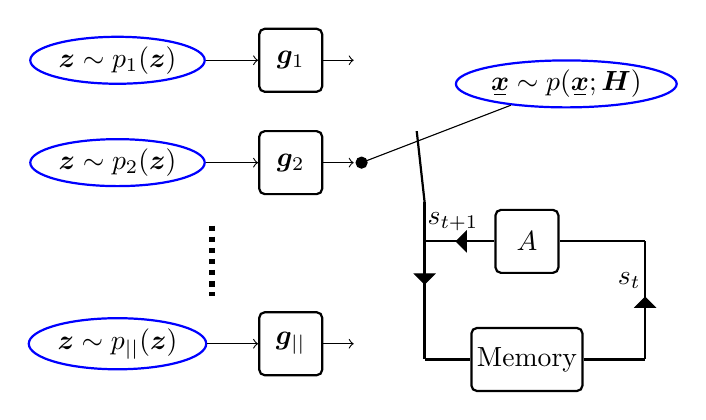
\begin{tikzpicture}
    \tikzstyle{enode} = [thick, draw=blue, ellipse, inner sep = 1pt,  align=center]
    % \tikzstyle{nnode} = [thick, rectangle, rounded corners = 1pt,minimum size = 1.2cm,draw,inner sep = 2pt]
    \tikzstyle{nnode} = [thick, rectangle, rounded corners = 2pt,minimum size = 0.8cm,draw,inner sep = 2pt]
    \node[enode] (z1) at (-1.2,1.8) {$\bm{z}\sim p_1(\bm{z})$};
    \node[nnode] (g1) at (1,1.8) {$\bm{g}_1$};

    \node[enode] (z2) at (-1.2,0.5){$\bm{z}\sim p_{2}(\bm{z})$};
    \node[nnode] (g2) at (1,0.5) {$\bm{g}_2$};

    \node[enode] (zK) at (-1.2,-1.8) {$\bm{z}\sim p_{|\Ss|}(\bm{z})$};
    \node[nnode] (gs) at (1, -1.8) {$\bm{g}_{|\Ss|}$};

    \node[enode] (x) at (4.5,1.5){$\ubm{x}\sim p(\ubm{x};\bm{H})$};
    % \node at (3,-1){$p(\bm{z}) = \sum_k\pi_kp_k(\bm{z})$};
        

    \draw[dotted,line width=2pt] (0,-0.3) -- (0,-1.2);
    \filldraw[->] (1.9, 0.5)circle (2pt) --  (x) ;
    \draw[->] (z1) -- (g1);
    \draw[->] (g1) -- (1.8, 1.8);

    \draw[->] (z2) -- (g2);
    \draw[->] (g2) -- (1.8, 0.5);

    % \draw[->] (1,-0.5) -- (1.8, -0.5);
    \draw[->] (zK) -- (gs);
    \draw[->] (gs) -- (1.8, -1.8);

    % \draw[->] (z1) [in=180,out=0]  to node[right]{$\pi_1$} (g);
    % \draw[->] (z2) [in=180,out=0]  to node[above]{$\pi_2$} (g);
    % \draw[->,dashed] (zK) [in=180,out=0]  to node[right]{$\pi_K$} (g);
    %\draw[->] (g) to (x);
    \begin{scope}[xshift=0.5cm, thick, every node/.style={sloped,allow upside down}]
      \node[nnode] (m) at (3.5,-2) {Memory};
      \node[nnode] (a) at (3.5,-0.5) {$A$};

      \draw (2.1,0.9)-- (2.2, 0.);
      \draw (2.2,0.)-- node {\midarrow} (2.2,-2);
      \draw (2.2,-2)-- (m);
      \draw (m)-- (5, -2);
      \draw (5, -2)-- node {\midarrow} (5 ,-0.5);
      \draw (5, -0.5) -- (a);
      \draw (a)-- node {\midarrow} (2.2, -0.5);
      \node at (4.8, -1) {$s_{t}$};
      \node at (2.56, -0.25) {$s_{t+1}$};
    \end{scope}
    
    

  \end{tikzpicture}
  \caption{GenM-HMM Model defined by $\bm{H} = \{\Ss, \bm{q}, A, p({\bm{x}}|{\bm{s}}; \bm{\Phi}) \}$}
  \vspace{0.1cm}
\end{figure}


For this proposal, we seek to use a generator mixed HMM scheme, termed as GenM-HMM. We define a set of generators for GenM-HMM:
\begin{equation}
  \{\bm{g}_{s}| s \in \Ss, \bm{g}_s: \bm{z}\rightarrow \bm{x}, \bm{z}\sim p_{s}(\bm{z})\}.
\end{equation}
Thus there are total $|\Ss|$ generators. $p(\bm{x}|{s}; \bm{\Phi})$ is induced as $\bm{g}_s(\bm{z}) \sim p(\bm{x}|{s}; \bm{\Phi})$ where $\bm{z} \sim p_s(\bm{z})$ for $s \in \Ss$. Let us denote the inverse of $\bm{g}_s$ as $\bm{f}_s = \bm{g}_s^{-1}$. We have the $s$-th component of the GenM-HMM model as
\begin{align}
  p(\bm{x} | s; \bm{\Phi})
  &= p_s(\bm{z}) \bigg| \det \left( \pd{\bm{z}}{\bm{x}} \right) \bigg| \nonumber \\
  &= p_s(\bm{f}_s(\bm{x})) \bigg| \det \left( \pd{\bm{f}_s(\bm{x})}{\bm{x}} \right) \bigg|
\end{align}
where $p_s(\bm{z})$ is the latent source distribution for $s=1, 2, \cdots, |\Ss|$.

Let us denote the parameter set that defines latent distribution $p_s(z)$ by $\bm{\omega}_s$ and the parameter set that defines generator $\bm{g}_s$ by $\bm{\theta}_s$. Then $\bm{\Phi} = \left\{ \bm{\theta}_s,
  \bm{\omega}_s, \forall s\in \Ss\right\}$. The problem in \autoref{eq:sub-gm} can be reformulated as:
\begin{align}
  &\umax{\bm{\Phi}} \Qq(\bm{\Phi}; \bm{H}^{\mathrm{old}}) \nonumber \\
  =&\umax{ \bm{\theta}_s, \bm{\omega}_s, \forall s\in \Ss} \sum_{r=1}^{R} \sum_{t=1}^{{T}^{(r)}-1} \sum_{\smtr{s}{t}{r}=1}^{|\Ss|}  p(\smtr{s}{t}{r}| \ubmr{x}{r}; \bm{H}^{\mathrm{old}}) \left[\log\,p_{\smtr{s}{t}{r}}(\bm{f}_{\smtr{s}{t}{r}}(\bmtr{x}{t}{r})) + \log\,\bigg| \det\, \left( \pd{\bm{f}_{\smtr{s}{t}{r}}(\bmtr{x}{t}{r})}{\bmtr{x}{t}{r}} \right) \bigg| \right].
\end{align}


The diagram of GenM-HMM is shown as follows.



\subsubsection{Latent-source Mixed HMM (LatM-HMM)}
\begin{figure}[!h]
  \centering
  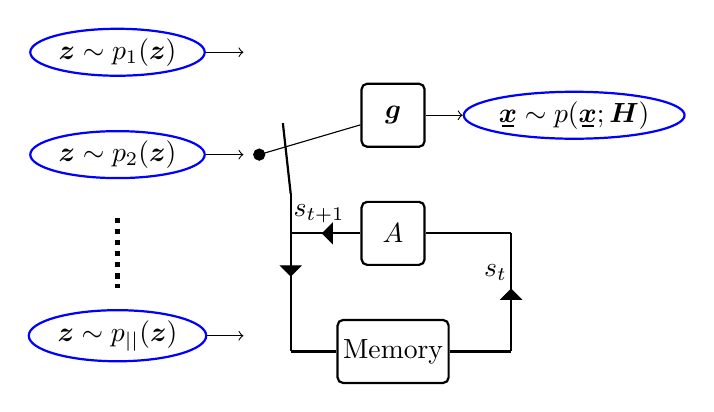
\begin{tikzpicture}
    \tikzstyle{enode} = [thick, draw=blue, ellipse, inner sep = 1pt,  align=center]
    % \tikzstyle{nnode} = [thick, rectangle, rounded corners = 1pt,minimum size = 1.2cm,draw,inner sep = 2pt]
    \tikzstyle{nnode} = [thick, rectangle, rounded corners = 2pt,minimum size = 0.8cm,draw,inner sep = 2pt]
    \node[enode] (z1) at (0,1.8) {$\bm{z}\sim p_1(\bm{z})$};
    \node[enode] (z2) at (0,0.5){$\bm{z}\sim p_{2}(\bm{z})$};
    \node[enode] (zK) at (0,-1.8) {$\bm{z}\sim p_{|\Ss|}(\bm{z})$}; 
    \node[enode] (x) at (5.8,1){$\ubm{x}\sim p(\ubm{x};\bm{H})$};
    % \node at (3,-1){$p(\bm{z}) = \sum_k\pi_kp_k(\bm{z})$};
    \node[nnode] (g) at (3.5,1) {$\bm{g}$};

    \node[nnode] (m) at (3.5,-2) {Memory};
    \node[nnode] (a) at (3.5,-0.5) {$A$};


    \draw[dotted,line width=2pt] (0,-0.3) -- (0,-1.2);
    \filldraw[->] (1.8, 0.5)circle (2pt) --  (g) ;
    \draw[->] (z1) -- (1.6, 1.8);
    \draw[->] (z2) -- (1.6, 0.5);
    % \draw[->] (1,-0.5) -- (1.8, -0.5);
    \draw[->] (zK) -- (1.6, -1.8);
    % \draw[->] (z1) [in=180,out=0]  to node[right]{$\pi_1$} (g);
    % \draw[->] (z2) [in=180,out=0]  to node[above]{$\pi_2$} (g);
    % \draw[->,dashed] (zK) [in=180,out=0]  to node[right]{$\pi_K$} (g);
    \draw[->] (g) to (x);
    \begin{scope}[ thick, every node/.style={sloped,allow upside down}]
      \draw (2.1,0.9)-- (2.2, 0.);
      \draw (2.2,0.)-- node {\midarrow} (2.2,-2);
      \draw (2.2,-2)-- (m);
      \draw (m)-- (5, -2);
      \draw (5, -2)-- node {\midarrow} (5 ,-0.5);
      \draw (5, -0.5) -- (a);
      \draw (a)-- node {\midarrow} (2.2, -0.5);
    \end{scope}
    \node at (4.8, -1) {$s_{t}$};
    \node at (2.56, -0.25) {$s_{t+1}$};

  \end{tikzpicture}
  \caption{LatM-HMM Model defined by $\bm{H} = \{\Ss, \bm{q}, A, p({\bm{x}}|{\bm{s}}; \bm{\Phi}) \}$}
  \vspace{0.1cm}
\end{figure}

Alternatively, we can use a latent-source mixed HMM (LatM-HMM) where different latent source share the same generator functioning as feature mapping. Then the generator of the LatM-HMM is defined as
\begin{equation}
  \left\{\bm{g}| \bm{g}: \bm{z}\rightarrow \bm{x}, s \in \Ss, \bm{z}\sim p_{s}(\bm{z})\right\}.
\end{equation}
We use $\bm{f} = \bm{g}^{-1}$ to denote inverse of $\bm{g}$ and use $\bm{\theta}$ to denote the parameter set of $\bm{g}$. Then the conditional probability for LatM-HMM is modeled as
\begin{align}
  p(\bm{x} | s; \bm{\Phi})
  &= p_s(\bm{z}) \bigg| \det \left( \pd{\bm{z}}{\bm{x}} \right) \bigg| \nonumber \\
  &= p_s(\bm{f}(\bm{x})) \bigg| \det \left( \pd{\bm{f}(\bm{x})}{\bm{x}} \right) \bigg|
\end{align}

The parameter set for this model to be decide is $\bm{\Phi} = \left\{ \bm{\theta},  \bm{\omega}_s, \forall s\in \Ss\right\}$.
Then the problem in \autoref{eq:sub-gm} can be reformulated as:
\begin{align}
  &\umax{\bm{\Phi}} \Qq(\bm{\Phi}; \bm{H}^{\mathrm{old}}) \nonumber \\
  =&\umax{ \bm{\theta}, \bm{\omega}_s, \forall s\in \Ss} \sum_{r=1}^{R} \sum_{t=1}^{{T}^{(r)}-1} \sum_{\smtr{s}{t}{r}=1}^{|\Ss|}  p(\smtr{s}{t}{r}| \ubmr{x}{r}; \bm{H}^{\mathrm{old}}) \left[\log\,p_{\smtr{s}{t}{r}}(\bm{f}(\bmtr{x}{t}{r})) + \log\,\bigg| \det\, \left( \pd{\bm{f}(\bmtr{x}{t}{r})}{\bmtr{x}{t}{r}} \right) \bigg| \right].
\end{align}



\textbf{To be continued}...
\section{On Implementation}
Found a HMM python lib that basics provide needed API for us, see \href{https://hmmlearn.readthedocs.io/en/stable/index.html}{hmmlearn}. Saikat also has suggestion.


For problem \autoref{eq:sub-gm} we are going to use our generative models to solve. I have the following consideration to revised our LatMM and GenMM for this application:
\begin{itemize}
\item Use factorized model instead of additive mixture model, to make likelihood computation logarithm domain compatible; 
\item Use full EM fashion instead of mini-batch fashion for training: store generative model as old for EM, there are always two neural networks working, one old for probability evaluation and one new for optimization.
\end{itemize}
\bibliographystyle{IEEEbib}

% \bibliography{bibliography}
\bibliography{myref}

% \appendix

% \input{section/sec-appendixA}
\end{document}


%%% Local Variables:
%%% mode: latex
%%% TeX-master: t
%%% End:
